%
% partabl.tex
%
% (c) 2021 Prof Dr Andreas Müller, OST Ostschweizer Fachhochschule
%
\documentclass[tikz]{standalone}
\usepackage{times}
\usepackage{amsmath}
\usepackage{txfonts}
\usepackage[utf8]{inputenc}
\usepackage{graphics}
\usetikzlibrary{arrows,intersections,math}
\usepackage{ifthen}
\begin{document}

\newboolean{showgrid}
\setboolean{showgrid}{false}
\def\breite{7}
\def\hoehe{4}

\definecolor{tangentenfarbe}{rgb}{0.8,0.4,0.8}
\definecolor{darkred}{rgb}{0.8,0,0}

\begin{tikzpicture}[>=latex,thick]
\clip (-6.3,-3.55) rectangle (6.3,3.55);

% Povray Bild
\node at (0,0) {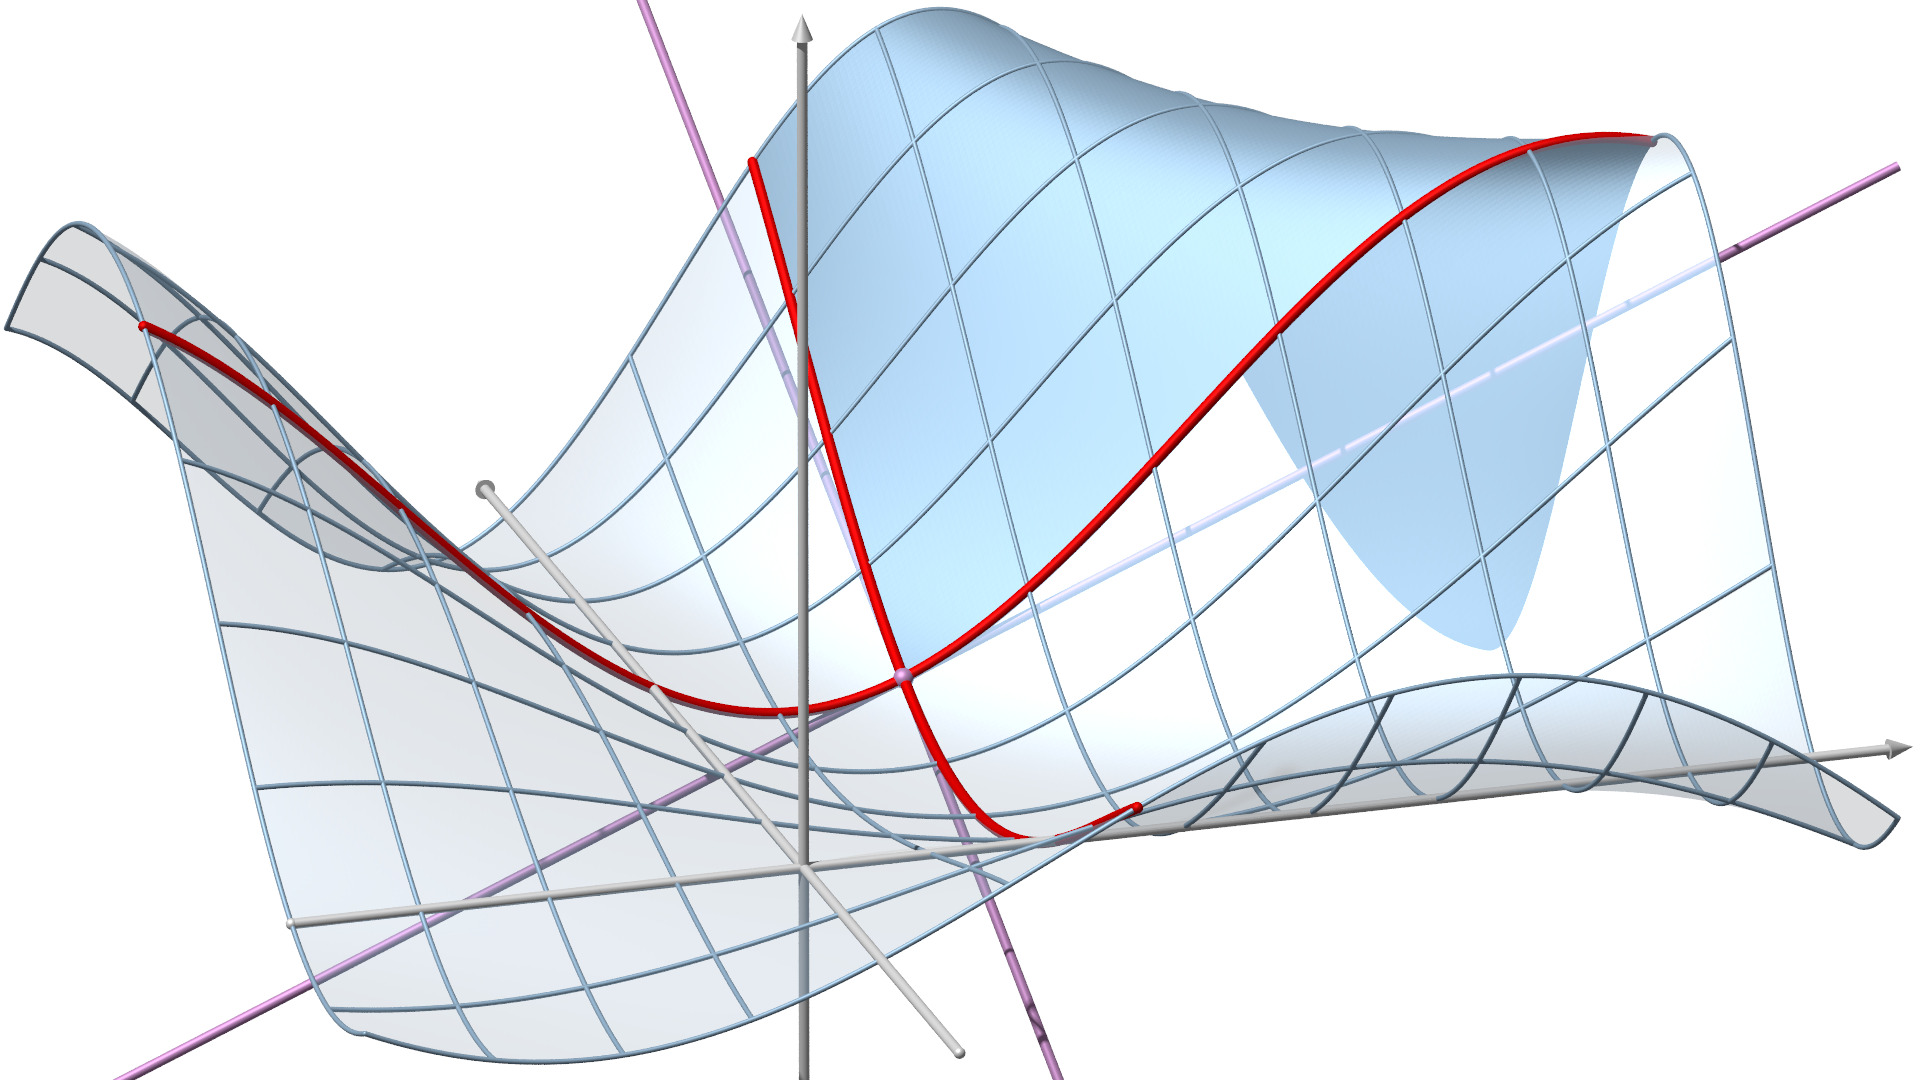
\includegraphics[width=12.6cm]{partabl.jpg}};

% Gitter
\ifthenelse{\boolean{showgrid}}{
\draw[step=0.1,line width=0.1pt] (-\breite,-\hoehe) grid (\breite, \hoehe);
\draw[step=0.5,line width=0.4pt] (-\breite,-\hoehe) grid (\breite, \hoehe);
\draw                            (-\breite,-\hoehe) grid (\breite, \hoehe);
\fill (0,0) circle[radius=0.05];
}{}

\node at (6.1,-1.1) {$x\mathstrut$};
\node at (-1.3,3.3) {$z\mathstrut$};
\node at (-3.1,0.6) {$y\mathstrut$};
\node[color=tangentenfarbe] at (-2.6,2.5)
	{$\displaystyle\frac{\partial f}{\partial y}(x_0,y_0)$};
\node[color=tangentenfarbe] at (5.6,2.7)
	{$\displaystyle\frac{\partial f}{\partial x}(x_0,y_0)$};
\node[color=darkred] at (1.4,-2.3) {$z=f(x_0,y)$};
\node[color=darkred] at (3,3) {$z=f(x,y_0)$};

\end{tikzpicture}

\end{document}

